\documentclass{beamer}


\usepackage[french,english]{babel}

\usepackage[T1]{fontenc}

\usepackage[utf8]{inputenc}


\usetheme{Warsaw}
\title{Nouvelle heuristique pour VRP}

\author{Clément Legrand}
\date{31 Mai 2018 \footnote{D'après l'article \emph{A simple, deterministic, and efficient knowledge-driven heuristic
for the vehicle routing problem} de Florian Arnold et Kenneth Sorensen}} 

\begin{document}

\section{Présentation heuristique}

\begin{frame}[plain]
\titlepage
\end{frame}

\begin{frame}{Description}
\underline{Intérêt}: heuristique simple à mettre en place, et performante.

\begin{block}{Etapes de l'algorithme:}
\begin{itemize}
\item Recherche solution initiale: Algorithme Clarke and Wright

\item Recherche de la "pire" arête

\item Optimisations locales ensuite par 3 opérateurs
\end{itemize}
\end{block}

\end{frame}

\section{Obtention de la pire arête}

\subsection{Caractériser une arête}

\begin{frame}{Comment caractériser une arête ?}
\begin{block}{Idée}
Trouver des liens entre les solutions (quasi-) optimales
\end{block}

Entraînement d'un modèle prédictif pour distinguer
les arêtes à supprimer des autres en s'aidant de caractéristiques:
\begin{itemize}
\item Largeur de la tournée
\item Profondeur de la tournée
\item Coût de la tournée
\end{itemize}

	\centering
	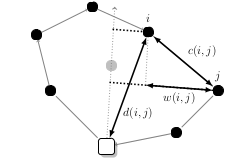
\includegraphics[height=0.4\textheight]{metrics.png}
	
\end{frame}

\subsection{Déterminer la pire arête}

\begin{frame}{Déterminer la pire arête}
Description spatiale précise d'une arête avec ces caractéristiques. 
\begin{center}
$b(i,j) = \frac{[\lambda_w w(i,j) + \lambda_c c(i,j)] [\frac{d(i,j)}{max_{k,l}d(k,l)}] ^ {\frac{\lambda_d}{2}}}{1+p(i,j)}$
\end{center}

\begin{itemize}
\item $p$ représente le nombre de fois où l'arête a été pénalisée (initialement 0)

\item Les paramètres $\lambda_w$,$\lambda_c$ et $\lambda_d$ valent $0$ ou $1$, et sont choisis selon le type d'instance.
\end{itemize}

\begin{exampleblock}{Pire arête}
La pire arête est celle qui maximise la fonction $b$.
\end{exampleblock}
\end{frame}

\section{Opérateurs locaux}

\subsection{Cross-exchange}

\begin{frame}{Cross-exchange}

\begin{block}{Objectif}
Essaie d'échanger deux séquences de clients entre deux tournées. 
\end{block}

\begin{alertblock}{Complexité}
Complexité en $O(n^4)$: beaucoup trop...
\end{alertblock}

	\centering
	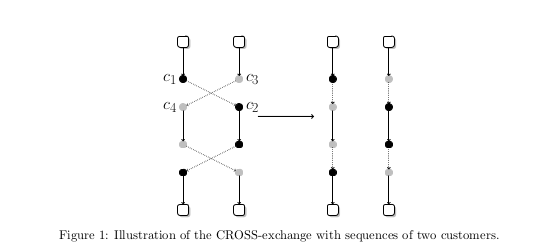
\includegraphics[height=0.4\textheight]{cross_exchange.png}
\end{frame}

\begin{frame}
\begin{exampleblock}{Algorithme}
\begin{itemize}
\item Choisir une arête $(c_1,c_2)$ à éliminer;
\item Trouver une autre tournée grâce aux voisins de $c_1$; (e.g. premier voisin sur une tournée différente $c_4$ , prendre arête $(c_3,c_4)$);
\item On échange $c_1$ et $c_3$;
\item On essaie d'échanger $s(c_4)$ avec $s(c_2)$, $s(s(c_2))$, ... jusqu'à trouver une amélioration ou avoir parcouru toute la tournée (dans ce cas on poursuit avec $s(s(c_4))$).
\end{itemize}
\end{exampleblock}

\begin{alertblock}{Nouvelle complexité}
$O(n^2)$ dans le pire cas, mais proche de linéaire en général.
\end{alertblock}
\end{frame}

\begin{frame}{Exemple}
Test de l'opérateur sur une tournée de 10 clients. L'arête rouge est l'arête à éliminer.

\begin{center}
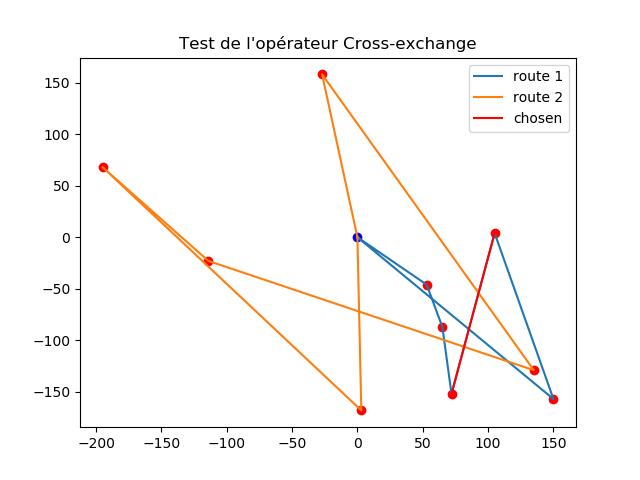
\includegraphics[scale=0.25]{test1CE_init.png}
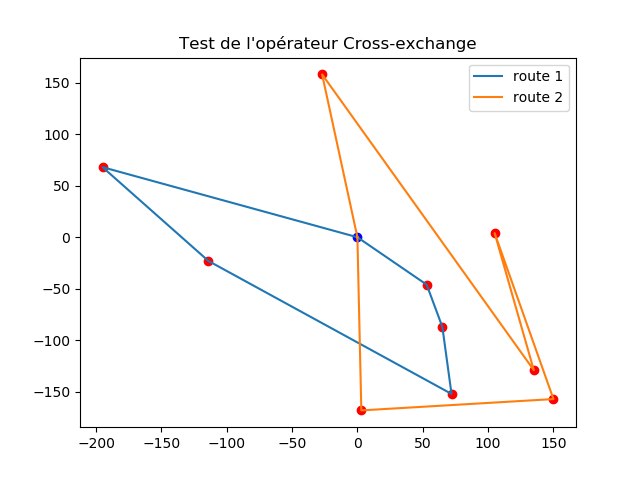
\includegraphics[scale=0.25]{test1CE_imp(corrige).png}
\end{center}

\end{frame}



\subsection{Ejection-chain}

\begin{frame}{Ejection-chain}

\begin{block}{Objectif}
Déplacer au plus $l$ clients sur des tournées plus adaptées. 
\end{block}

\begin{exampleblock}{Algorithme}
\begin{itemize}
\item Déterminer une arête à éliminer; considérer un des deux clients;
\item Regarder parmi les pp-voisins pour trouver une tournée;
\item Déplacer le client sur cette tournée;
\item Essayer de déplacer un client de cette tournée sur une autre tournée, tel que le saving soit maximal;
\item Recommencer l'étape précédente $l$ fois; On applique les changements si le saving final est positif.
\end{itemize}
\end{exampleblock}

\end{frame}

\begin{frame}

\begin{alertblock}{Complexité}
Complexité en $O(n^{l-1})$. En pratique $l=3$. 
\end{alertblock}

	\centering
	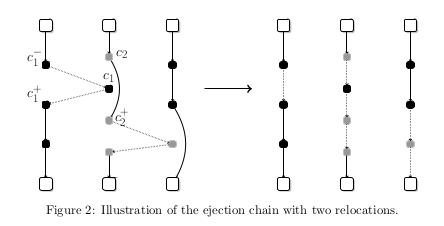
\includegraphics[height=0.4\textheight]{ejection_chain.png}
\end{frame}


\subsection{Lin-Kernighan Heuristic}
\begin{frame}{Lin-Kernighan Heuristic}

\begin{block}{Utilisation}
\begin{itemize}
\item Utilisé en général pour TSP;
\item Optimisation intra-tournée (chaque tournée est améliorée indépendamment des autres).
\end{itemize}
\end{block}

\begin{exampleblock}{Algorithme}
\begin{itemize}
\item Exécute i-opt (échange l'ordre de $i$ clients sur la tournée; au départ $i=2$).
\item Si $i=k$ ou plus d'améliorations possibles $\rightarrow$ réalise la meilleure i-opt; recommence avec $i=2$
\item Si amélioration possible $\rightarrow$ recommence avec $i+1$
\item Si $i=2$ et pas d'améliorations possibles $\rightarrow$ on sort de la boucle.
\end{itemize}
\end{exampleblock}

\end{frame} 

\begin{frame}
\begin{alertblock}{Complexité}
Complexité en $O(n^k)$, $k$ choisi par l'utilisateur. En général $k=2$.
\end{alertblock}

\begin{center}
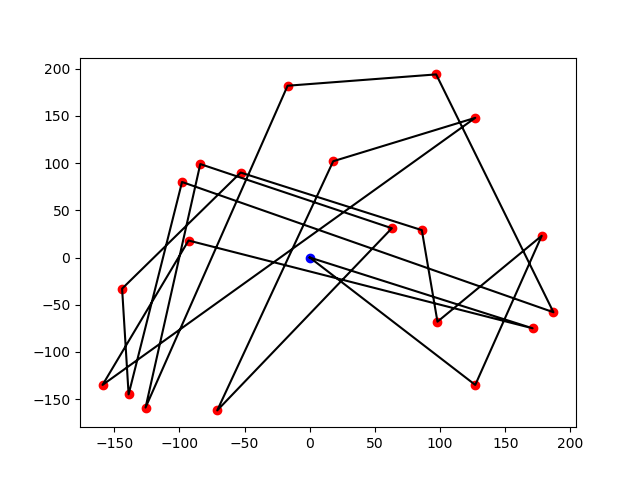
\includegraphics[scale=0.32]{test4_20_init.png}
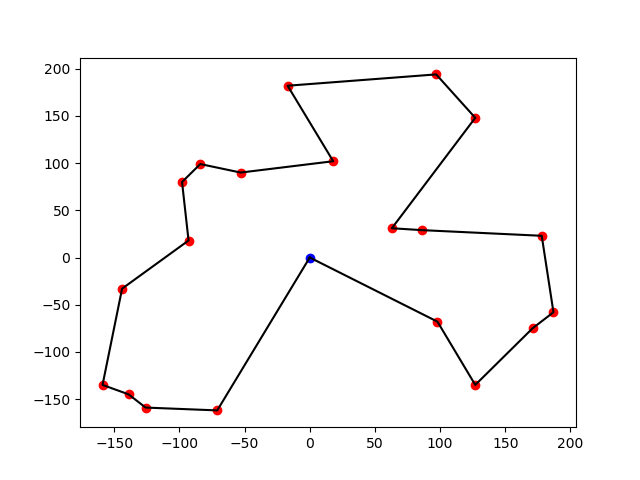
\includegraphics[scale=0.32]{test4_20_LKopt.png}
\end{center}

\end{frame}


\section{Améliorations}

\begin{frame}{Que faire si on ne trouve plus d'améliorations ?}
\begin{block}{Idées}

\begin{itemize}
\item Optimisation globale (application des opérateurs sur l'ensemble du graphe): très coûteux
\item Remise à zéro des pénalités
\item Changement de la fonction de pénalisation
\end{itemize}

\end{block}
\end{frame}

\begin{frame}{Résultats actuels}
Implémentation de l'heuristique.
Test sur 100 clients, passage de $6443$ (CW) à $5214$ (fin heuristique).
\begin{center}
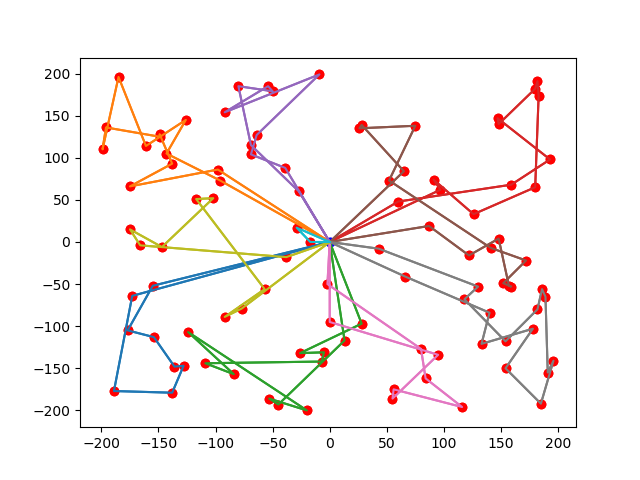
\includegraphics[scale=0.32]{test2_heuristic_init.png}
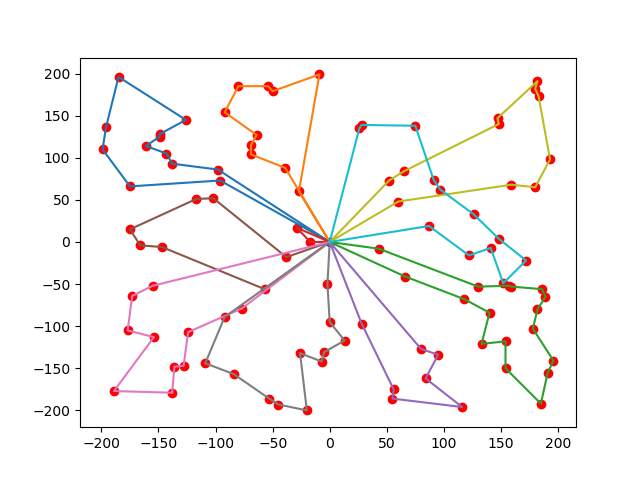
\includegraphics[scale=0.32]{test2_heuristic_res.png}
\end{center}
\end{frame}

\end{document}